\section{Consuntivazione}

\subsection{Milestones:}
\begin{itemize}
    \item Release versione 0.0.4 (Completa al: 80\%)
\end{itemize}

\subsection{Attività svolte}

\begin{table}[ht]
    \begin{tabularx}{\textwidth}{X l l}
        
        \rowcolor{gray!30} \textbf{Attività} & \textbf{Stato} & \textbf{Ruolo}\\
        
        \hline
        aggiunti processi primari alle \textbf{Norme di Progetto} & completato & Amministratore\\
        aggiunti processi di supporto alle \textbf{Norme di Progetto} & completato & Amministratore\\
        definite norme di codifica & completato & Amministratore\\
        documentato il \textbf{PoC} & completato & Amministratore\\
        progredito con il \textbf{PoC}& completato & Amministratore\\
        \end{tabularx}
    \caption{Lista delle attività svolte durante lo sprint}
\end{table}


\begin{table}[ht]
    \begin{tabularx}{\linewidth}{X|rrrrrrr}
    \rowcolor{gray!30}& Re & Amm & An & Pro & Prog & Ver & tot \\
    \hline
    Bonavigo Michele                        & 2,4 & 1,7 & 0 & 0 & 0 & 0,45  & 4,55 \\
    \rowcolor{gray!10}Casarotto Mattia      & 0 & 0 & 8,9 & 0 & 0 & 0 & 8,9 \\
    Massarenti Alessandro                   & 0,4 & 5,95 & 5,75 & 0 & 0 & 1  & 13,1 \\
    \rowcolor{gray!10}Peron Samuel          & 0 & 0 & 0 & 0 & 0 & 0 & 0 \\
    Pierobon Luca                           & 0 & 0 & 0,35 & 0 & 0 & 3,9 & 4,25 \\
    \rowcolor{gray!10}Romano Davide         & 0 & 0 & 0 & 0 & 0 & 0 & 0 \\
    Zarantonello Giorgio                    & 0 & 0 & 4,5 & 0 & 0 & 0 & 4,5 \\
    \hline                                  & 2,8 & 7,65 & 19,5 & 0 & 0 & 5,35 & 
    \end{tabularx}
    \caption{\label{ruoli-persone}Spartizione dei ruoli e ore svolte durante lo sprint}
\end{table}

\begin{center}
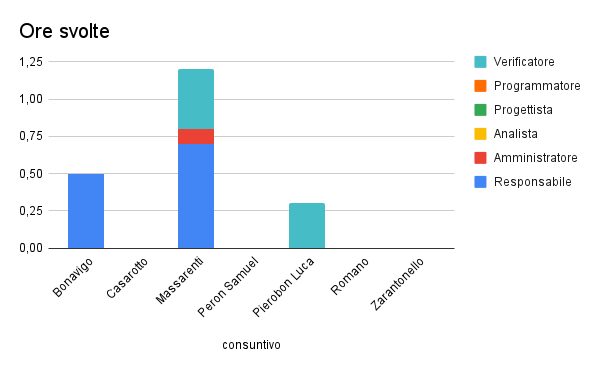
\includegraphics[width=12cm]{img/ore-svolte.png}
\end{center}

\begin{table}[ht]
    \begin{tabularx}{\linewidth}{X|l|l}
    \rowcolor{gray!30}& Ore & Costo \\
    \hline
    
    Responsabile & 2,8 & € 84,00 \\
    \rowcolor{gray!10}Amministratore & 7,65 & € 153,00 \\
    Analista & 19,5 & € 487,50 \\
    \rowcolor{gray!10}Progettista & 0 & € 0,00 \\
    Programmatore & 0 & € 0,00 \\
    \rowcolor{gray!10}Verificatore & 5,35 &€ 80,25 \\
    totale & 35,3 & € 804,75 \\
    \end{tabularx}
    \caption{\label{costi-ruolo}Spartizione dei ruoli e ore svolte durante lo sprint}
\end{table}


Avendo quindi consumato €804,75\footnote{Si veda tabella \ref{costi-ruolo}} del budget durante questo sprint, rimangono ancora a disposizione € 11836,00 per gli sprint seguenti.

\subsection{Trend e riflessioni}

\begin{figure}[ht]
    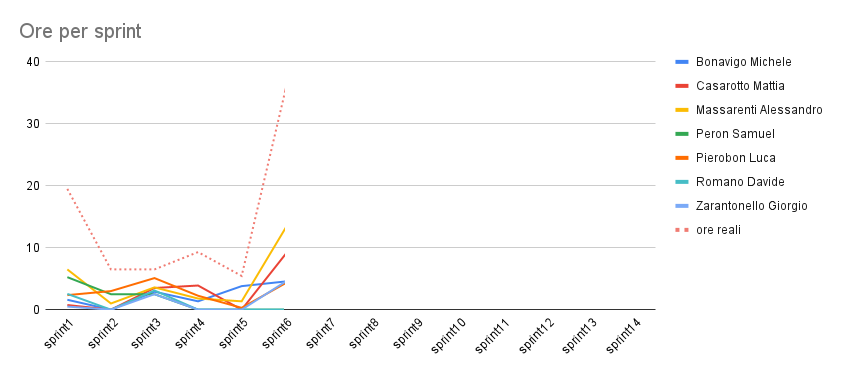
\includegraphics[width=\linewidth]{img/andamento.png}
    \caption{Andamento ore utilizzate nei vari sprint}\label{img:andamento}
\end{figure}

Come preventivato nel verbale SPR\_20230101, ovvero quello precedente, possiamo notare nella figura \ref{img:andamento} un trend positivo.

È nostro desiderio mantenere questo ritmo.

\subsection{Difficoltà e problemi di sprint}

Alcune questioni sono risultate durante questo sprint:

\begin{itemize}
    \item il proponente non ha ancora definito il supporto hardware per i lampioni aa cui dovremo far fede.
\end{itemize}

Queste verranno discusse in sede di preparazione del prossimo sprint.
